% ==============================================================================
% ==============================================================================
%
%        CHOOSE ONE OPTION BY ALTERNATING THE COMMENTED-OUT LINE
%           For the order of .tex files, open controller.tex
%
% ==============================================================================
% ==============================================================================

% OPTION 1: Manuscript Style

\documentclass[fleqn]{article}

% OPTION 2: Journal Style

% \documentclass[twocolumn,twoside,fleqn]{article}


% ==============================================================================
% ==============================================================================
%
%                      DO NOT MODIFY BEYOND THIS POINT
%
% ==============================================================================
% ==============================================================================


% PACKAGES
% ------------------------------------------------------------------------------

\usepackage{simplemargins}
\usepackage{tocloft}
\usepackage[T1]{fontenc}
\usepackage{textcomp}
\usepackage{setspace}
\usepackage[round,authoryear,semicolon]{natbib}
\usepackage{ifthen}
\usepackage{ifpdf}
\usepackage{titling}
\usepackage{titlesec}
\usepackage{units}
\usepackage{amsbsy}
\usepackage{caption}
\usepackage{subfig}
\usepackage{balance}
\usepackage{times}
\usepackage[hang]{footmisc}


% MARGINS AND DIMENSIONS
% ------------------------------------------------------------------------------

\settopmargin{0.70in}
\setleftmargin{0.55in}
\setrightmargin{0.56in}
\setbottommargin{1in}
\addtolength{\oddsidemargin}{0.17in}
\addtolength{\textwidth}{-0.17in}
\footnotemargin 1em
\setlength{\mathindent}{0in}
\setlength{\parindent}{0.24in}


% PDF FIGURES
% ------------------------------------------------------------------------------

\ifpdf
	\usepackage{graphicx}
	\usepackage[pdftex,bookmarks=false]{hyperref}
\else
	\usepackage{graphics}
	\usepackage{graphicx}
	\usepackage{epsfig}
	\usepackage[dvipdfm,bookmarks=false]{hyperref}
\fi


% ORPHANS AND WIDOWS
% ------------------------------------------------------------------------------

\clubpenalty=10000
\widowpenalty=10000


% LINKS
% ------------------------------------------------------------------------------

\hypersetup{
    pdfpagelayout=OneColumn,
	colorlinks = true,
	urlcolor   = blue,
	citecolor  = blue,
	linkcolor  = blue
}
\urlstyle{same}


%  CAPTIONS
% ------------------------------------------------------------------------------

\captionsetup{font={footnotesize,sf},labelfont=bf}
\captionsetup[subfloat]{font={scriptsize,sf},textfont=scriptsize}

\newcommand{\sublabel}[2]{\raisebox{#1in}{\sffamily\scriptsize\bfseries(#2)}}


% HEADERS AND FOOTS
% ------------------------------------------------------------------------------

\makeatletter
\if@twocolumn
    \usepackage{fancyhdr}
	\setlength{\columnsep}{0.33in}
	\renewcommand{\headrulewidth}{0pt}
	\fancyhf{}
    \fancyfoot[RO]{
        \usefont{T1}{phv}{c}{n}\small
        Seismological Research Letters \hspace{1em} Volume 00, Number 0 \hspace{1em} November/December 2016 \hspace{1em} \thepage}
    \fancyfoot[LE]{
        \usefont{T1}{phv}{sb}{n}\small
        \thepage \hspace{1em} Seismological Research Letters \hspace{1em} Volume 00, Number 0 \hspace{1em} November/December 2016}
\else
	\usepackage[left,displaymath,pagewise]{lineno}
	\setlength\linenumbersep{20pt}
	\doublespacing
	\captionsetup{font=doublespacing}
	\cftpagenumbersoff{figure}
	\usepackage[tablesfirst,notablist]{endfloat}
	\AtBeginDelayedFloats{\renewcommand\baselinestretch{1.4}}
	\renewcommand\cftloftitlefont{\large}
	\renewcommand\listfigurename{
		\begin{center}
		Figure Captions
		\end{center}
	}
	\setlength{\cftparskip}{2ex}
	\renewcommand\cftfigpresnum{\bf Figure~}
	\renewcommand\cftfigaftersnum{.}
	\renewcommand\cftfignumwidth{5.5em}	
\fi
\makeatother


% SECTION FORMATS COMMANDS
% ------------------------------------------------------------------------------

\titleformat{\section}{\raggedright}{}{0pt}{\usefont{T1}{phv}{bc}{n}\large\uppercase}
\titlespacing*{\section}{0pt}{10pt}{10pt}

\titleformat{\subsection}{\raggedright}{}{0pt}{\usefont{T1}{phv}{bc}{n}\normalsize}
\titlespacing*{\subsection}{0pt}{10pt}{0pt}

\renewcommand{\refname}{REFERENCES}


% ADDITIONAL COMMANDS
% ------------------------------------------------------------------------------

% 
\newcommand{\sublabel}[2]{\raisebox{#1in}{\sffamily\scriptsize\bfseries(#2)}}

% Earthquake macros
% -----------------

\newcommand{\dt}{$\Delta t$}
\newcommand{\vs}{$V_{\mathrm{s}}$}
\newcommand{\mathvs}{V_{\mathrm{s}}}
\newcommand{\vp}{$V_{\mathrm{p}}$}
\newcommand{\mathvp}{V_{\mathrm{p}}}
\newcommand{\vseq}[1]{$V_{\mathrm{s}}=#1$~m/s}
\newcommand{\vsgeq}[1]{$V_{\mathrm{s}}\geq#1$~m/s}
\newcommand{\vsleq}[1]{$V_{\mathrm{s}}\leq#1$~m/s}
\newcommand{\vpeq}[1]{$V_{\mathrm{p}}=#1$~m/s}
\newcommand{\vsmin}{$V_{\mathrm{s}_{\min}}$}
\newcommand{\vsmineq}[1]{$V_{\mathrm{s}_{\min}}=#1$~m/s}
\newcommand{\vsminleq}[1]{$V_{\mathrm{s}_{\min}}\leq#1$~m/s}
\newcommand{\vsmingeq}[1]{$V_{\mathrm{s}_{\min}}\geq#1$~m/s}
\newcommand{\fmax}{$f_{_{\max}}$}
\newcommand{\mathfmax}{f_{_{\max}}}
\newcommand{\fmaxeq}[1]{$f_{_{\max}}=#1$~Hz}
\newcommand{\fmaxgeq}[1]{$f_{_{\max}}\geq#1$~Hz}
\newcommand{\fmaxleq}[1]{$f_{_{\max}}\leq\;$#1~Hz}
\newcommand{\eqmag}[1]{$M_{\mathrm{#1}}$}
\newcommand{\eqmageq}[2]{$M_{\mathrm{#1}}=#2$}
\newcommand{\eqmagleq}[2]{$M_{\mathrm{#1}}\leq#2$}
\newcommand{\eqmaggt}[2]{$M_{\mathrm{#1}}>#2$}
\newcommand{\tenexp}[2]{$#1\times 10^{#2}$}
\newcommand{\qs}{$Q_{\mathrm{s}}$}
\newcommand{\qp}{$Q_{\mathrm{p}}$}
\newcommand{\mathqs}{Q_{\mathrm{s}}}
\newcommand{\mathqp}{Q_{\mathrm{p}}}


% Math macros
\newcommand{\pepsi}{\epsilon^{p}}
\newcommand{\dpepsi}{\dot{\epsilon}^{p}}
\newcommand{\eepsi}{\epsilon^{e}}
\newcommand{\deepsi}{\dot{\epsilon}^{e}}
\newcommand{\depsi}{\dot{\epsilon}}

% Reference equations with parenthesis
% ------------------------------------

\newcommand{\refeqn}[1]{Equation \ref{#1}}

% Reference figures
% -----------------

\newcommand{\reffig}[1]{Fig.~\ref{#1}}
\newcommand{\refFig}[1]{Figure~\ref{#1}}


% Easy volume and area
% --------------------

\newcommand{\vdomain}[4]{#1~#4 $\times$ #2~#4 $\times$ #3~#4}
\newcommand{\adomain}[3]{#1~#3 $\times$ #2~#3}

% Title and sections fonts and style
% ----------------------------------

\titleformat{\section}{\raggedright}{}{0pt}{\usefont{T1}{phv}{bc}{n}\large\uppercase}
\titlespacing*{\section}{0pt}{10pt}{10pt}

\titleformat{\subsection}{\raggedright}{}{0pt}{\usefont{T1}{phv}{bc}{n}\normalsize}
\titlespacing*{\subsection}{0pt}{10pt}{0pt}

\renewcommand{\refname}{REFERENCES}
%\titleformat{\bibname}{\raggedright}{}{0pt}{\usefont{T1}{phv}{bc}{n}\large\uppercase}


%\titleformat{\subsection}{}{}{1.5em}{\normalsize}
%
%\titleformat{\subsubsection}[runin]{}{}{0pt}{\normalsize\itshape}[.]

% Manuscript tricks
% -----------------

\newcommand\manuscriptadjust{
\makeatletter
\ifthenelse{\boolean{@twocolumn}}{}{~\clearpage}
\makeatother
}

\newcommand\preprintadjust{
\makeatletter
\ifthenelse{\boolean{@twocolumn}}{\small}{}
\makeatother
}

% Figure and Table captions configuration
% ---------------------------------------

%\captionsetup[table]{
%%	labelfont=large,
%	labelsep=newline,
%	justification=centerlast,
%	textfont=small
%}
%\captionsetup[figure]{
%	labelfont=bf,
%	labelsep=period,
%	textfont=small
%}

\makeatletter
\if@twocolumn
    \newcommand\introduction{\section{Introduction}}
\else
    \newcommand\introduction{
        \linenumbers
	    \section{Introduction}}
\fi
\makeatother


%\newcommand\corresponding{%
%	\makeatletter
%	\if@twocolumn
%	\else
%	   \thanks{Corresponding author.}
%	\fi
%    \makeatother
%}%

\newcommand{\myaffil}[1]{$^{\mbox{\small #1}}$}




\newcommand\manuscriptadjust{
\makeatletter
\ifthenelse{\boolean{@twocolumn}}{}{~\clearpage}
\makeatother
}

\newcommand\preprintadjust{
\makeatletter
\ifthenelse{\boolean{@twocolumn}}{\small}{}
\makeatother
}

\newcommand{\myaffil}[1]{$^{\mbox{\small #1}}$}
\newcommand{\cmmnt}[1]{}

% TITLE AND AUTHORS PREPARATION
% ------------------------------------------------------------------------------

\pretitle{
    \vspace{-30pt}
    \begin{flushleft}
    \usefont{T1}{phv}{bc}{it}
    \Huge
}

\posttitle{
    \end{flushleft}
}

\preauthor{
    \begin{flushleft}
    \vspace{3pt}
    \usefont{T1}{phv}{bc}{n}
    \LARGE
}

\postauthor{
    \end{flushleft}
    \vspace{0.3em}
}

\predate{
    \begin{flushleft}
    \makeatletter
	\vspace{-3em}
}

\postdate{
    \if@twocolumn
    \else
    	~\clearpage
    \fi
	\section{Abstract}
	\vspace{-2.6em}
    \end{flushleft}
}

% Revision format added 
\usepackage[dvipsnames]{xcolor}
\newcommand{\myrevision}[1]{\textcolor{Green}{#1}}

% ==============================================================================
% THE DOCUMENT
% ==============================================================================


% TITLE AND AUTHORS INPUT
% ------------------------------------------------------------------------------


\title{%
    Analysis of 2005--2015 Earthquake Sequence in Northern Iran Using the Visibility Graph Method
}

\makeatletter
\if@twocolumn
    \date{}
    \renewcommand*\@fnsymbol[1]{\the#1}
    \author{by Naeem Khoshnevis, Shima Azizzadeh-Roodpish, Ricardo Taborda, and Luciano Telesca}
\else
    \author{
        Naeem Khoshnevis,\myaffil{1,$\ast$} Shima Azizzadeh-Roodpish,\myaffil{1,2} Ricardo Taborda\myaffil{1,2} and Luciano Telesca\myaffil{3}\\
        \normalsize\normalfont    	    	
        \vspace{20pt}
        1.~
        Center for Earthquake Research and Information\\
        \hspace{1.1em} The University of Memphis, Memphis, TN 38152, U.S.A.\\
        \vspace{20pt}
        2.~
        Department of Civil Engineering\\
        \hspace{1.1em} The University of Memphis, Memphis, TN 38152, U.S.A.\\
        \vspace{20pt}
        3.~
        Institute of Methodologies for Environmental Analysis\\
        \hspace{1.1em} National Research Council, Tito, Italy\\
        \vspace{20pt}
        *.~
        Corresponding author\\
        \hspace{1.1em} Email: nkhshnvs@memphis.edu\\
        \vspace{40pt}
    }
\fi
\makeatother




% START DOCUMENT STRUCTURE
% ------------------------------------------------------------------------------

\begin{document}


% PAGE STYLE
% ------------------------------------------------------------------------------

\makeatletter
\if@twocolumn
    \pagestyle{fancy}
\fi
\makeatother

\maketitle
\makeatletter
\if@twocolumn
    \thispagestyle{fancy}
\fi
\makeatother





% ABSTRACT
% ------------------------------------------------------------------------------

\noindent
\begin{abstract}
The seismicity of northern Iran between 2005 and 2015 is investigated by means of visibility graph (VG) method. In this study the northern Iran is divided into three tectonic seismic regions: Azerbaijan, Alborz, and Kopeh Dagh.  The aftershocks and foreshocks are removed from the catalog and the magnitude time series are generated for each tectonic seismic zone. Using declustered catalog, we studied the VG properties of the magnitude time series. The results show a relationship between the $k-M$ slope and the $b-value$ of the Gutenberg-Richter law. Topological properties (i.e. $< T_c >$, $k-M$ slope) of network and  dynamic properties of magnitude time series (i.e. $b-value$) significantly decrease before large earthquakes. Combining  the results of this study with two similar previous studies, improves the linear correlation coefficient factor and empower the idea of universal relationship between $b-value$ and $k-M$ slope. The behavior of  the VG's properties are similar to previous studies and could be considered an alternative method for analyzing the earthquake sequence. 
\end{abstract}


% ------------------------------------------------------------------------------


\makeatletter
\if@twocolumn
    \vspace{2em}
\fi
\makeatother


% MAIN CONTENT
% ------------------------------------------------------------------------------



\section{Introduction}
\noindent
\citet{Lacasa2008} presented a simple and fast computational method; known as visibility algorithm, to convert the time series into the graphs. Basically the visibility graph presents the connection between nodes in the network. In each time series two characteristics are attributed to each incidents, including the time and the value of the incident. Two events are connected to each other, or visible to each other, if there is not any other event to interrupt their linear connection. In mathematical form, event $i$ and event $j$ are visible to each other if the following equation fulfills:

\begin{equation}
\frac{y_i - y_k }{t_k - t_i} > \frac{y_i - y_j}{ t_j - t_i} 
\end{equation}

\noindent
where, $y$ is the value of the event and $t$ is the time of the event. $k$ is the index of any event between event $i$ and event $j$. 

\noindent
The visibility graph that is generated from the time series holds the following conditions, 1) each event is visible to the events at the right and left side (if there is any) of the event  (Connectivity), 2) The algorithm is developed without defining a direction for the links (Undirected),  3) Rescaling or translation of the time series are not changing the resulted visibility graph (Invariant under affine transformations of  the series data)\citep{Lacasa2008}.

\noindent
The analysis of seismicity sequence through visibility graph for various tectonic seismic regions, revealed an alternative approach to study the magnitude time series. \citet{Telesca2012} studied the seismic sequence of Italy between 2005 and 2010 through using the visibility graph method. Using different threshold magnitude, and observing the collapsing effect of all the distribution degrees, they argued that in analyzing the magnitude time series, VG seems to depend only on the values of the magnitude and independent of the threshold magnitude. In other study, \citet{Telesca2013} studied the Seismicity of the Mexican subduction zone through visibility graph approach. They extracted the characteristics of the visibility graph for five different tectonic seismic regions.  According to their study visibility graph could identify one of the regions that has a different seismicity characteristics, which is because of different tectonic processes that governs the area. The relationship between Gutenberg-Richter parameters and $k-M$ slope (The slope of regression line of Magnitude  of each event $(M)$ and its connectivity degree $k$) is investigated in their study. In a similar study \citet{Telesca2014}, studied the seismicity of 2002-2011 Pannonian seismicity using the visibility graph. They classified seismic catalog into shallow and deep earthquakes and extract the visibility graph characteristics for each class. According to their study there is close relationship between Gutenberg-Richter $b-value$ and $k-M$ slope of the visibility graph. High linear correlation coefficient of $b-value$ and $k-M$ slope suggests the universal character of the relationship between these parameters \citep{Telesca2014}.  \citet{Telesca2016} , used the $ <T_C>$, as the parameter window mean interval connectivity time ,  that indicates the mean linkage time between earthquakes, to study the 2003-2012 earthquake sequences in the Kachchh region of western India. They found that the $<T_C>$ changes through time, indicating that the topological properties of the earthquake network are not stationary; also $<T_C>$ significantly decrees before the largest shock of the catalog. Analyzing Gutenberg-Richter values of  magnitude time series of an earthquake sequence revealed more opportunities to study the magnitude time series using the features of networks. \\

\noindent
In this study we used visibility graph analysis to study the earthquake sequence of northern Iran. We divided northern Iran into three tectonic seismic regions including Azerbaijan, Alborz, and Kopeh Dagh.  Recently, northern Iran has been studied in detail from different seismological points of view. \citet{Nemati2015} studied the most recent 200 years' seismicity in northern Iran. The frequency of shocks vary widely from one main shock per 6 years (0.17 event/ year) for the Azerbaijan region to 13 earthquakes per 4 years for the Kopeh-Dagh (3.25 event/year) region. \\

\noindent
Northern Iran has an elaborate seismic history.  Having considerable number of earthquake and also being in different seismic tectonic zone, northern Iran is a good platform to analysis the visibility graph method's capabilities for studying the magnitude time series. In this study we present the relationship between $K-M$ slope and the $b-value$ in three different tectonic seismic region. We also investigate the variation of $<T_C>$ value through time.





\section{Seismicity of Northern Iran}

We are interested in applying the visibility graph method to analyze the seismicity of northern Iran. This region is part of the Iranian plateau, on the Himalayan-Alpine seismic belt. It is confined by the relative movements between the Arabian, Eurasian, eastern Asia-Minor, and Indian plates; and has a long history of large magnitude ($M>7$) earthquakes that are well documented dating back to the eight century \citep[e.g.,][]{Berberian_1981_Chap}. According to the tectonic settings and geologic provinces of the plateau, the seismic activity in Iran has been categorized into different seismic zones. These vary between four to nine major seismic zones, in the more traditional models \citep[e.g.,][]{Stocklin1968, Takin1972, Berberian1976}, up to twenty to twenty-three seismotectonic provinces in the most elaborate ones \citep[e.g.,][]{Nowroozi1976, Tavakoli1999}. We adopt the model proposed by \citet{Mirzaei1998} with modifications introduced by \citet{Karimiparidari2013}. In it, Iran is divided into six seismic regions: Azerbaijan, Alborz, Kopeh Dagh, Zagros, Central-East Iran, and Makran. Our focus, however, is on the northern part of Iran, for which we define a region of interest between longitudes 43.5\textdegree{}E and 61.5\textdegree{}E, and latitudes 34\textdegree{}N and 40\textdegree{}N, as shown in Fig.~\ref{fig:study_region}. Although this region encloses part of the Zagros and Central-East seismic zones, we concentrate in the analysis of the seismicity of Azerbaijan, Alborz and Kopeh Dagh.

\begin{figure*}[t]
	\centering
	\includegraphics[width=\textwidth]{figure-02} 
	\caption{Region of interest, highlighting the seismic zones that are the focus of this study: Azerbaijan, Alborz, and Kopeh Dagh. The top-right location-map shows Iran and the selected area with respect to neighboring countries. The solid dark lines show the boundaries of the additional Zagros and Central-East seismic zones. This zonation follows the division proposed by \citet{Mirzaei1998} and later modified by \citet{Karimiparidari2013}. The background shows fault lines and the shaded relief. The color version of this figure is available only in the electronic edition.}
	\label{fig:study_region}
\end{figure*}

Northern Iran houses about 41 percent (32 million) of the total population of the country, and has suffered devastating earthquakes in the past \citep[e.g.,][]{Mehrain_1990_Tech, Chafory-Ashtiany_1999_DPM, Razzaghi_2012_Tech}. At the northwest, the seismic zone of Azerbaijan is strongly controlled by the North Tabriz Fault system in the vicinity of the city of Tabriz, shown in Fig.~\ref{fig:study_region}. Historical accounts document the occurrence of strong $M>6$ earthquakes in this region as far back as the ninth century \citep{Berberian1999}, and a few $M>7$ earthquakes in 1042, 1721 and 1780 \citep{Jones1834}. More recently, this region was struck by the $M_w$ 6.1 1997 Ardabil earthquake near the city of Ardabil and the $M_w$ 6.4 2012 Tabriz earthquake northeast of the city of Tabriz. These earthquakes caused extensive damage and took the lives of more than 1,500 people. 

The seismicity in the north-central region of Alborz is dominated by multiple fault systems, including the Talesh, Rubdar, North Alborz, and North Tehran faults, which also have a history of producing strong ground shaking. According to \citet{Ambraseys_1982_Book}, Tehran was devastated by severe $M>7$ earthquakes in 743, 958, 1177, 1665, and 1830. This region has also seen some significant recent seismic activity \citep{Berberian1999}, including the $M_w$ 7.4 1990 Manjil-Rudbar earthquake, which caused numerous deaths and damage to the region in the south Caspian depression, south from the city of Rasht and northwest from Tehran. 

Last, there is the Kopeh Dagh seismic zone to the east and northeast. This region is dominated by the Main Kopeh Dagh Fault system, which exhibits active tectonic displacements along a distance of more than 500 km \citep{Trifonov1978}. This fault is responsible for the $M_w$ 7.3 1948 earthquake, which struck the capital city of Ashgabat in Turkmenistan and destroyed more than 30 villages in Iran. Historically, the Kopeh Dagh seismic zone is also responsible for the $M_s$ 7.1 earthquake in 10 A.D.~\citep{Berberian2001} near Ashgabat, and two significant earthquakes in 1209 and 1405 at the boundary between the Neyshabur and Binalud faults near the city of Mashhad \citep{Berberian1999}.

\begin{figure*}[t]
	\centering
	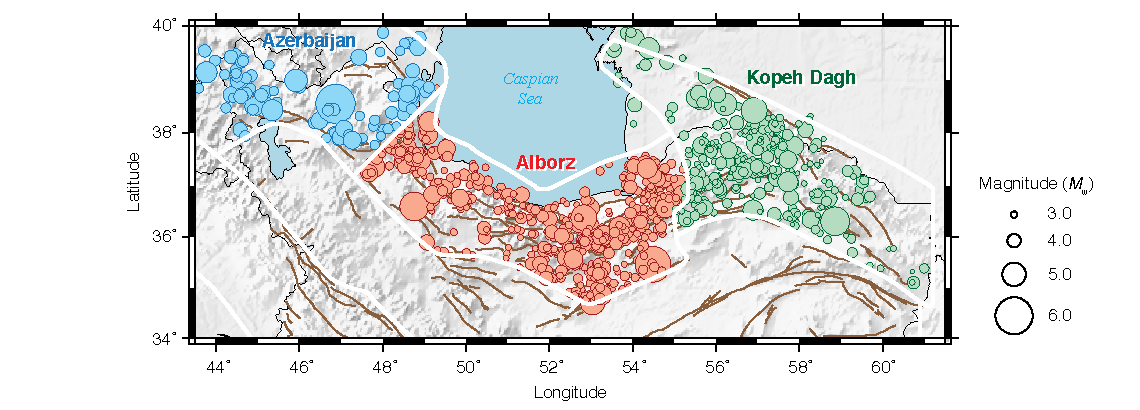
\includegraphics[width=\textwidth]{figure-03} 
	\caption{Declustered instrumental seismicity of northern Iran for the 2005--2015 period, considering only the events in the seismic zones of interest, namely Azerbaila, Alborz, and Kopeh Dagh. The size of symbols are proportional to the magnitude of the events, as indicated by the artificial scale shown on the right. The background shows fault lines and the shaded relief. The color version of this figure is available only in the electronic edition.}
	\label{fig:seismicity}
\end{figure*}

It follows from this description that the region of interest is one of significant seismic activity, which goes back centuries. We are, however, interested in the most recent instrumental seismicity. In particular, we focus on events recorded in the last decade, between January 2005 and December 2015. We focus our analysis on this magnitude-time sequence period because in a previous study we observed that the latest decade of seismic records in northern Iran offered the most complete dataset of recorded events, especially for the case of small $M < 4$ earthquakes \citep[e.g.][]{Khoshnevis2016}.

We compiled a catalog of all recorded earthquakes using data downloaded from the International Institute of Earthquake Engineering and Seismology, IIEES (see the Data and Resources section). The obtained dataset contained a mixture of earthquake magnitude scales, including: moment, $M_w$; local, $M_L$; body wave, $m_b$; surface wave, $M_s$; and duration $M_D$ magnitudes. We converted all earthquakes to moment magnitude, $M_w$. Magnitudes in the $M_L$, $m_b$, and $M_s$ scales were converted using the relationships defined in \citet{Zare2014}, whereas $M_D$ magnitudes were converted using the empirical relationship proposed by \citet{Deniz2010}.

Foreshocks and aftershocks were removed from the catalog following a Poissonian occurrence model using the declustering method of \citet{Gardner1974}, in a manner consistent with previous catalog compilations available for the region \citep[e.g.,][]{Zare2014}. Upon declustering, we divide the catalog into three sub-catalogs, each for one of the seismic zones under consideration. Fig.~\ref{fig:seismicity} shows the epicenter location of declustered instrumental earthquakes for the three seismic zones of interest.

We then proceeded to determine the minimum magnitude of completeness, $M_c$, for each region's sub-catalog. The value of $M_c$ is often determined using simple numerical analyses in combination with data inspection. Two common approaches are the maximum curvature (MAXC) and the goodness-of-fit test (GFT) methods \citep{Wiemer2001}. We use the GFT method as introduced by \citet{Wiemer2000}. In this method, the completeness magnitude is obtained such that the catalog satisfies---at a certain acceptance threshold---the Gutenberg-Richter power low, given an extended dataset of events. This extended dataset is composed of predicted and observed events, where the predicted events are generated based on a trial minimum magnitude. The process is repeated for increasing values of the reference minimum magnitude until finding a desirable fit with the power law. \citet{Wiemer2000} suggests a goodness of fit of 90\% as an acceptable threshold to select $M_c$. However, not all frequency-magnitude distributions reach the 90\% mark, in which case $M_c$ can be selected by inspection. 

Figure \ref{fig:completeness} shows the goodness-of-fit values for the three seismic zones. We indicate the selected value of $M_c$ for each region in the figure. We also obtained the $b$-value in the Gutenberg-Richter law for each region following the maximum likelihood estimation \citep{Aki1965}:
% 
\begin{equation}
	b = \frac{log_{10}(e)}{\overline{M} - M_{min}} \, ,
\end{equation}
% 
where $e$ is the mathematical constant or Euler's number, $\overline{M}$ is the average magnitude, and $M_{\min}$ is the minimum magnitude in the sample. Here, the value of $M_{\min}$ is taken as the minimum completeness magnitude $M_c$ obtained or selected for each region's sub-catalog. Table \ref{tab:seismicity} shows the corresponding values of $M_c$ and $b$.

\begin{figure}%[t]
	\centering
	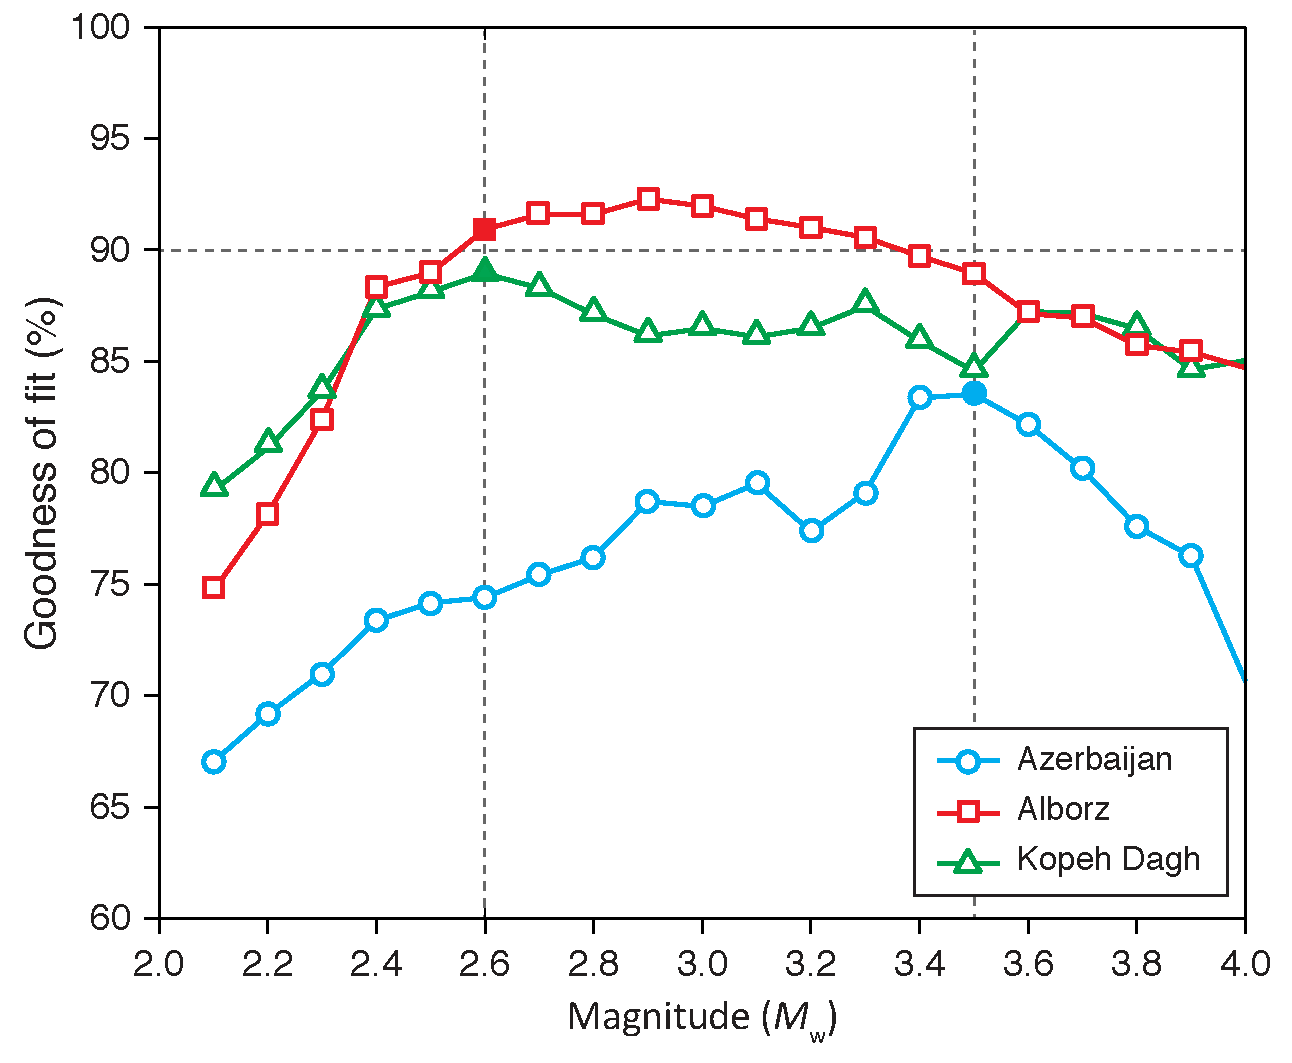
\includegraphics[width=0.45\textwidth]{figure-04} 
	\caption{Completeness magnitude goodness-of-fit test (GFT) results and selected $M_c$ values for the three tectonic seismic regions in northern Iran as evaluated from the time-magnitude sequence of earthquakes during the 2005--2015 period. The symbols indicate the computed GFT values as function of the earthquake magnitude. The horizontal dashed line indicates the desired threshold for the GFT value at 90 percent. The vertical dashed lines and solid symbols indicate the selected completeness magnitude for each region. The color version of this figure is available only in the electronic edition.}
	\label{fig:completeness}
\end{figure} 

\begin{table}
	\fontfamily{lmss}\selectfont
	\caption{Total and declustered number of earthquakes and seismic parameters $M_c$ and $b$ for the three seismic zones of northern Iran.}
	\centering\small
	\begin{tabular}{|ccccc|}
		\hline
		Region      & Total Num. & Declus.~Num. & \textit{M}c & \textit{b}-value \\ 
		            & of Events  & of Events &             &                  \\
		\hline
		Azerbaijan  &        271 &        93 &         3.5 &             1.02 \\
		Alborz      &       1262 &       794 &         2.6 &             0.77 \\
		Kopeh Dagh  &        399 &       282 &         2.6 &             0.58 \\
		\hline
	\end{tabular}
	\label{tab:seismicity}
\end{table}

\begin{figure*}[t]
	\centering
	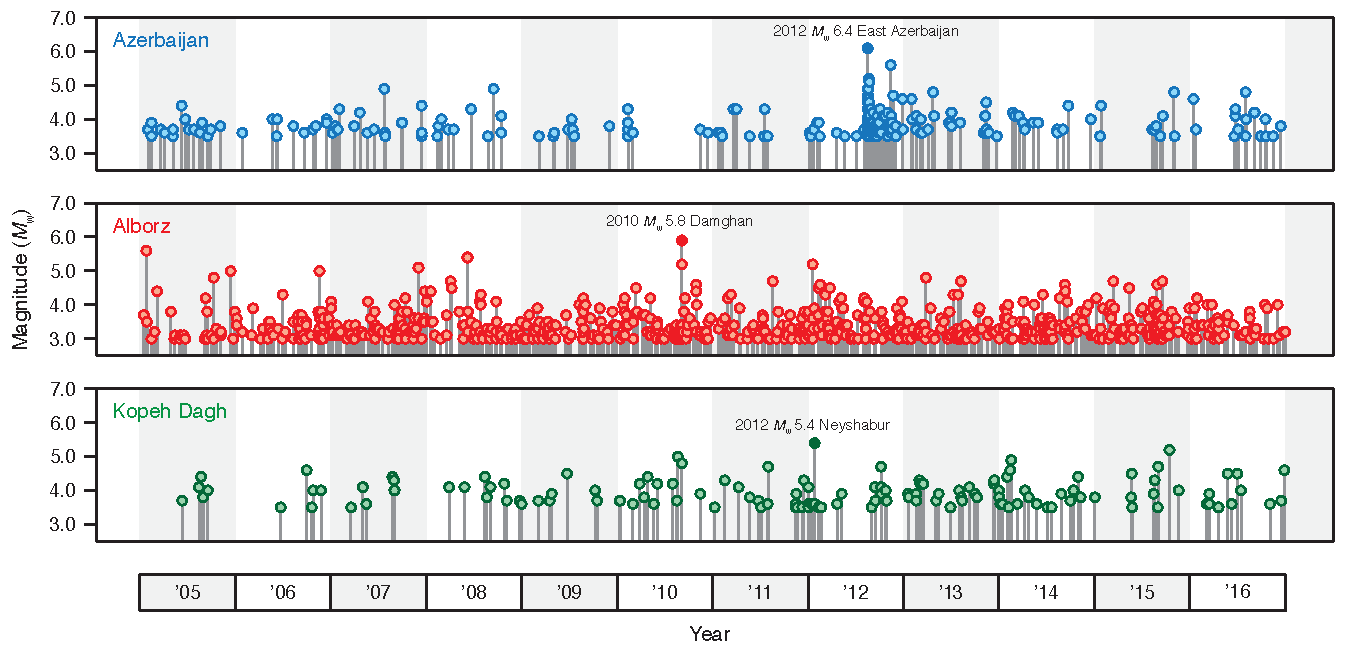
\includegraphics[width=\textwidth]{figure-05} 
	\caption{Time-magnitude sequences for the northern Iran seismic zones of Azerbaijan, Alborz and Kopeh Dagh, during the period between 1 January 2005 and 31 December 2015. The event occurrences are represented by vertical bars or sticks of length equal to the $M_w$ magnitude of each earthquake. These sequences correspond to the declustered catalog but in each case we consider only events with $M_w \geq M_c$. As shown in Fig.~\ref{fig:vg}, the dots at the top of each stick represent the nodes of the visibility graphs. The edges or links are omitted for visual convenience. Highlighted in the figure are the largest events in each sub-catalog, namely the 2012 $M_w$ 6.4 East Azerbaijan, 2010 $M_w$ 5.8 Damghan, and 2012 $M_w$ 5.4 Neyshabur earthquakes. The color version of this figure is available only in the electronic edition.}
	\label{fig:mag-time}
\end{figure*}

In addition to using $M_c$ to determine the $b$-value for each sub-catalog, we also use $M_c$ as the threshold for limiting the minimum magnitude to be considered in the construction of the visibility graph of each region. The resulting number of events for each region is included in Table \ref{tab:seismicity}. Figure \ref{fig:mag-time} shows the final time-magnitude sequences for Azerbaijan, Alborz and Kopeh Dagh. Note that in the case of Alborz and Kopeh Dagh, we consider events in the declustered catalog down to $M_w \geq 2.6$, whereas in the case of Azerbaijan all events are $M_w \geq 3.5$.




\section{Results}

We generate the visibility graphs for each subregion of interest using the time-magnitude sequences \myrevision{of both the complete and declustered catalogs. In the case of the complete catalog, that corresponds to the sequences shown in Fig.~\ref{fig:mag-time}. In every case, the numbers of nodes in each graph are the same as those shown in Table \ref{tab:seismicity}; and} the links between inter-visible events are established following the condition in equation (\ref{eq:vg}), as in the example shown in Fig.~\ref{fig:vg}. (We do not include a visualization of the graphs because the links are so many, that it is only practical to visualize the graphs of short sequences.) We collect information about the number of inter-visibility links associated with each event (connectivity degree, $k$) and categorize the events in magnitude bins of size $\Delta M_{\mathrm{bin}} = 0.1$, as mentioned in the Methodology section. Figure \ref{fig:km} shows the scattered distribution of events in the magnitude-connectivity degree plane for each subregion\myrevision{, corresponding to the complete catalogs.} The figure shows that, in general, the value of $k$ increases with $M_w$\myrevision{; and includes the results of obtaining linear $k$-$M$ regressions for each dataset along with the values of the slope $m$ for the three seismic zones, namely 10.05, 9.85, and 8.71 for the Azerbaijan, Alborz, and Kopeh Dagh regions. Similar results regressions were obtained for the declustered catalogs, which yielded $m$ values of 8.92, 8.97, and 7.96, respectively.}

\begin{figure*}[t]
	\centering
	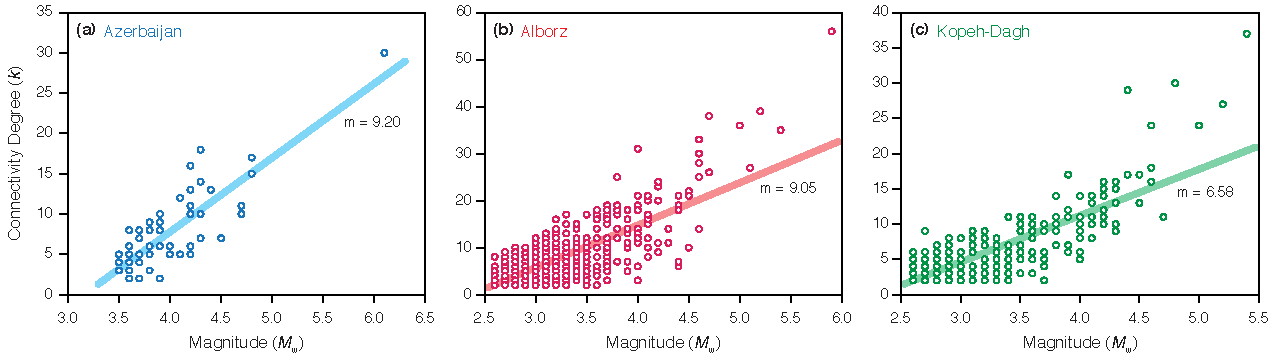
\includegraphics[width=\textwidth]{figures/pdf/figure-06} 
	\caption{Scattered distribution of events in the magnitude-connectivity degree plane and linear regressions obtained for the $k$-$M$ relationships for the three seismic regions in northern Iran. The value next to each of regression line corresponds to the slope of the line, which is referred here as the $k$-$M$ slope.}
	\label{fig:km}
\end{figure*}

Next, we examine the relationship between the $b$ values from Table \ref{tab:seismicity} and the $k$-$M$ slopes. \myrevision{Figures \ref{fig:regression}a and \ref{fig:regression}b show the scattered results of the $m$ versus $b$ for the complete and declustered catalogs, respectively. Along with the data-points obtained for our analysis of the three seismic regions of northern Iran, in each plot, we also include the data points corresponding to the magnitude-time sequences of the Mexican subduction zone provided by \citet{Telesca2013}, the Pannoninan seismic zone from \citet{Telesca2014}, the experimental results obtained by \citet{Telesca2014-pone}, and the result from a similar preliminary analysis done by \citet{Azizzadeh_2017_SSA} for California. These figures also include the linear trends of the data points, as they are aggregated (i.e., each regression reflects the addition of new data-points from different studies). In the figure, we indicate which data points were considered for each of the computed linear regressions and their corresponding correlation coefficient, $R$.}

\myrevision{Here, as well as in other figures, we present our results for both the complete and declustered catalogs to shed light upon the local differences for the case of northern Iran, and to contribute, globally, to the discussion of the appropriate treatment and selection of catalogs for the use of the visibility graph method. We note, for instance, that the data points in Fig.~\ref{fig:regression} from \citet{Telesca2012} and \citet{Telesca2013} used whole catalogs, whereas those from \citet{Telesca2014} and \citet{Telesca2016} used declustered catalogs.}

\myrevision{Note that, overall, the linear trends shown in Fig.~\ref{fig:regression} hold independently of the differences in the studies in terms of number of events, seismic characteristics, and the treatment of the catalogs. Also note that these trends tend to improve with increasing number of data points, as reflected by the increasing value of $R$. Regarding this, we should note that the data points in Fig.~\ref{fig:regression} cover what would otherwise be considered a large span of $b$ values. While we recognize that most earthquake data lead to $b$ values ranging between 0.8 and 1.2, it is also known that there are regions with low- and high-$b$ values \citep[e.g.,][]{Singh_1983_BSSA, Pacheco_1992_N, Nakaya_2006_JGR}. In addition, \citet{Scholz_1968_BSSA} reported that experimental microfractures in rocks, similar to those observed in earthquakes, exhibit $b$ values ranging between 0.11 and 2.58. Considering that, by definition, $b$ represents the proportion between the amount of large and small events in a region, the trends shown in Fig.~\ref{fig:regression} contribute to the suggestion made by \citet{Telesca2014} about the universal character of the relationship between $b$ and $m$.}

According to these results, a universal relationship between $b$ and $m$ can be expressed as
% 
\begin{equation}
\myrevision{
	b = 0.073 + 0.084 m
	\label{eq:universal.bm}
}
\end{equation}
%
\myrevision{for the case in which we consider the complete catalogs for northern Iran, and}
% 
\begin{equation}
\myrevision{
	b = 0.077 + 0.085 m
	\label{eq:universal.bm.dc}
}
\end{equation}
%
\myrevision{for the case in which we consider the declustered catalogs for northern Iran. This indicates that once combined with the data points of other regions, the option of considering either catalog leads to very similar results as, on average, the data points oscillate about the same universal relationship. Locally, however, for the case of northern Iran trends alone, it seems that the declustered catalog leads to a closer fit with the universal relationship. Separately (not shown here for brevity), we also observed that, for the particular sequences under study, the results seem to be more sensitive to less conservative values of $M_c$, as the choice of a smaller $M_c$ leads to larger datasets. \citet{Telesca2012} and \citet{Telesca2013}, however, pointed out that for sufficiently long sequences, the threshold magnitude have only small effects on the graph parameters.}

\begin{figure*}[t]
	\centering
	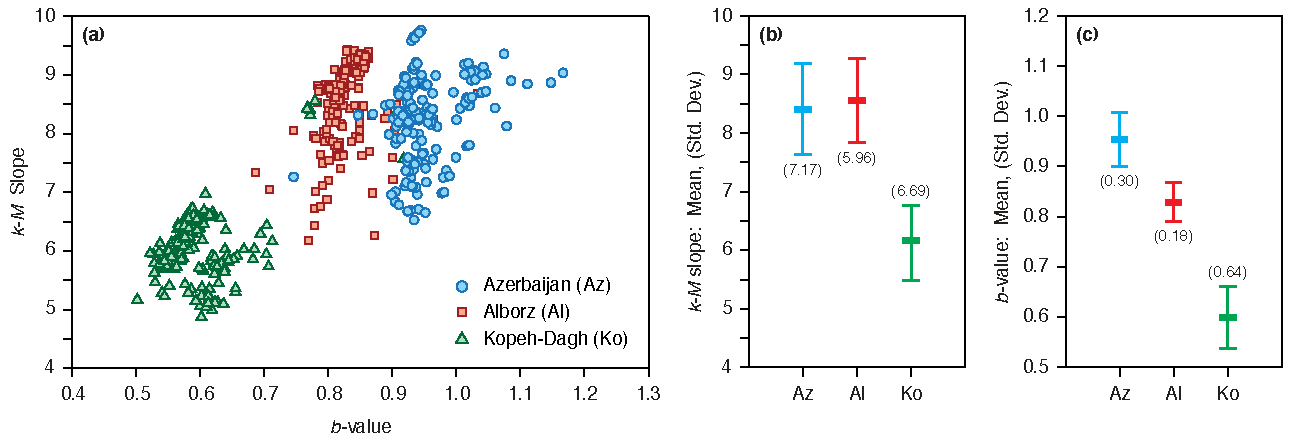
\includegraphics[width=\textwidth]{figures/pdf/figure-07} 
	\caption{\myrevision{Correlation between $k$-$M$ slope ($m$) and the $b$ value as drawn from the results of the present study for the region of northern Iranian using the complete (a) and declustered (b) catalogs, along with other previous studies including analysis of the Mexican subduction zone \citep{Telesca2013}, the Pannonian seismic zone \citep{Telesca2014}, southern California \citep{Azizzadeh_2017_SSA}, and results from two experiments \citep{Telesca2014-pone}. The lines represent linear regressions obtained to fit the different data points, considering different combinations. The values of the correlation coefficient, $R$, are indicated for each regression line.}}
	\label{fig:regression}
\end{figure*}

To further explore the sensitivity of the graph properties to the number of events in each catalog and the value of the minimum magnitude, we randomly picked a significant number of subsequences from within the initial catalog compiled for each region, and repeated the analysis for each subsequence. In total, for each region, we extracted 200 new subsequences from the \myrevision{whole} catalog. The number of events in each subsequence, $n$, was varied randomly but chosen to be large enough to represent the seismic characteristics of each region. In particular, the minimum size of each subsequence was set to be \myrevision{$n \geq 200$}, and the maximum size in the sequence was set to be as large as the original \myrevision{whole} catalog (see Table \ref{tab:seismicity}). We forced the random subsequences to progress positively in time without altering the natural occurrence of events. In other words, we randomly determined the initial event and the subsequence size (number of events to be considered), and then picked that number of events following the initial earthquake in the subsequence. Next, we determined the value of $M_c$ and $b$ \myrevision{to obtain the complete and declustered catalogs for each region}, created the graph for all events with $M \geq M_c$, and extracted the connectivity degree of the events in each subsequence. \myrevision{Because this needed to be done for a large number of subsequences, in this part of the analysis we used the goodness-of-fit test (GFT) method to determine $M_c$ systematically, instead of the MAXC method. The GFT method follows the recommendations of \citet{Wiemer2000} and \citet{Wiemer2001}, and leads to less conservative values of $M_c$, which is preferable to keep the subsequences large enough.}

\begin{figure*}%[t]
	\centering
	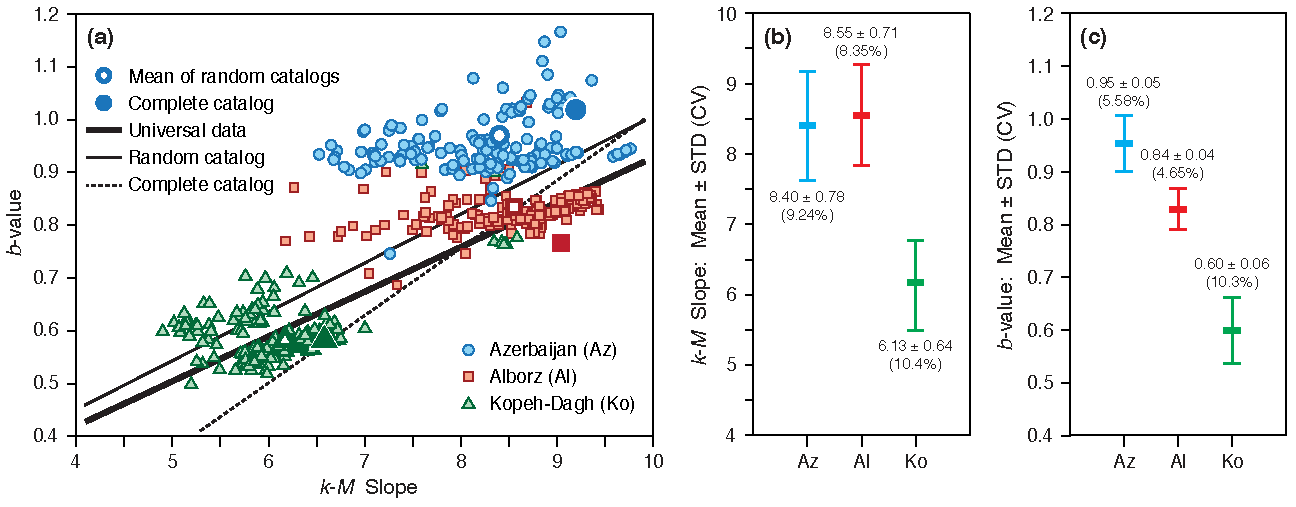
\includegraphics[width=\textwidth]{figures/pdf/figure-08} 
	\caption{\myrevision{Correlation between the $k$-$M$ slope ($m$) and $b$ values for the random subsequences extracted from the catalogs of the three northern Iranian seismic regions considered in this study (scattered symbols, 200 each region, 600 total) for both the complete (a) and declustered (d) catalogs, including the mean values (empty symbols with thick border) and the data points obtained from the regional analyses (solid symbols), along with the linear regressions of each sample as indicated in the legend; and mean $\pm1$ standard deviation bar plots for $m$ (b,e) and $b$ (c,f) for the complete and declustered catalogs, respectively. In the latter, the values in the parentheses corresponds to the coefficients of variation.}}
	\label{fig:random}
\end{figure*}

\myrevision{Fig.~\ref{fig:random} shows the results for this analysis on random subsequences for both the complete and declustered catalogs. In particular, Figs.~\ref{fig:random}a and \ref{fig:random}d show} scattered points for all the individual $m$ and $b$ pairs for all the subsequences that were randomly picked from the \myrevision{complete and declustered} catalogs of each region in northern Iran (small symbols)\myrevision{, respectively}. Figures \ref{fig:random}b \myrevision{and \ref{fig:random}e show the variability of $m$, and Figs.~\ref{fig:random}c and \ref{fig:random}f show the variability of $b$. These variability plots} show the mean values of each parameter for all the random subsequences and the amplitudes of $\pm 1$ standard deviation, as well as the coefficients of variation (in percentage). \myrevision{Figures \ref{fig:random}a and \ref{fig:random}d also include the data points corresponding to the regional analysis of the catalogs, the points corresponding to the mean values of $m$ and $b$, and the universal linear regression from equations (\ref{eq:universal.bm}) and (\ref{eq:universal.bm.dc}), as well as the linear regressions for northern Iran when using the full-sequence catalogs (dashed thin line) and the random subsequence catalogs (continuous thin line).}

\myrevision{In essence, the results in Fig.~\ref{fig:random} show that, despite the variability in the random subsequences and the differences in the computation of $M_c$, both of which are sources of additional uncertainty, the analysis produces an outcome in fair agreement with the universal relationships. Nonetheless, the analysis of the random subsequences in the complete catalogs produces some outliers, whereas the processing of the declustered subsequences tends to concentrate more evenly around the universal trend. Note that, likely due to the removal of foreshocks and aftershocks, the declustered random subsequences exhibit a clearer distinction between the three seismic zones.}

\myrevision{While these sequences do not represent the dominant seismicity pattern of the region, the comparison between the mean values of the random sequences analysis versus the complete catalogs (large, empty and solid symbols in Fig.~\ref{fig:random}) indicates that there exists only a small bias, which is well within the standard deviation of the different value samples. Note also that the values of $m$ in Fig.~\ref{fig:random} are slightly smaller when obtained with the random sequence analysis than when done for the regional sequences, whereas the $b$ values seem more stable. This explains why the regressions of the random subsequences are less steep than the universal regressions, in both cases. In a separate initial analysis, not included here for brevity, we observed that lower, less conservative selections of $M_c$ can lead to random subsequences that yield regressions in better agreement with the universal trend. Using lower values of $M_c$, however, may be misleading. In this sense, larger catalogs in better instrumented regions may shed light on the stability of the $m$-$b$ relationship, which is the reason we included the data point from \citet{Azizzadeh_2017_SSA} for southern California in Fig.~\ref{fig:regression}, which falls well in line with the universal regression.}

\begin{figure*}%[t]
	\centering
	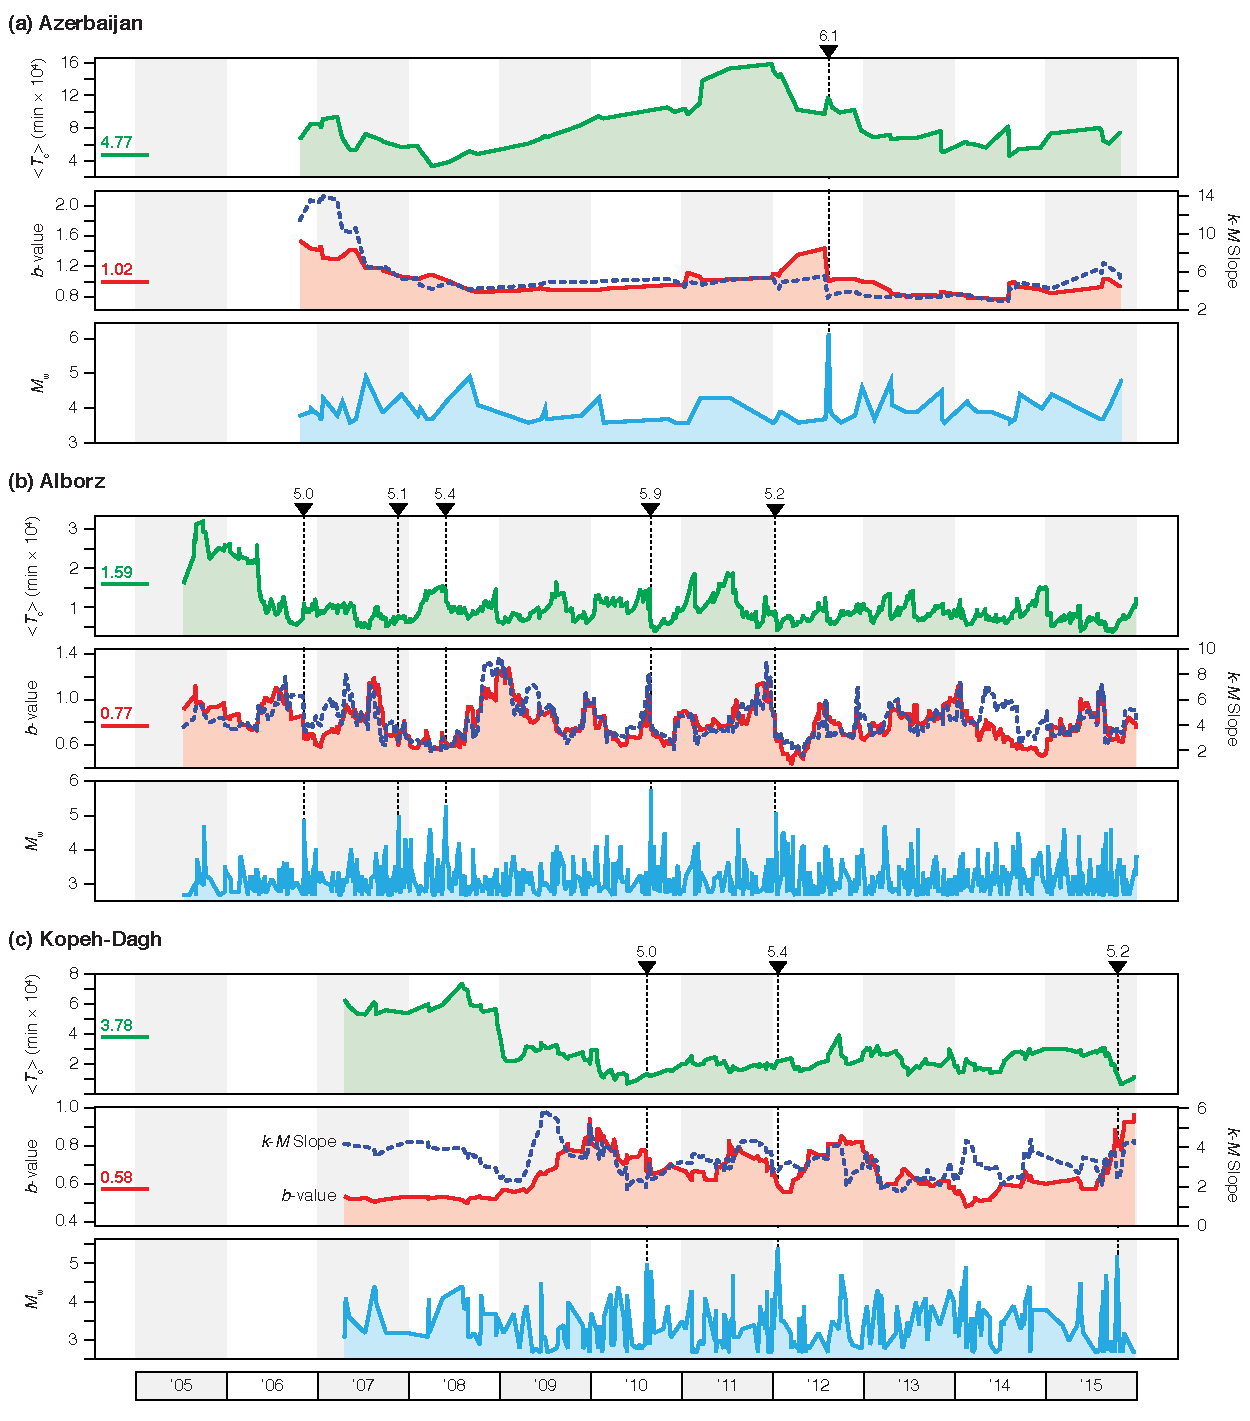
\includegraphics[width=\textwidth]{figures/pdf/figure-09} 
	\caption{\myrevision{Variation of $<$$T_c$$>$, $k$-$M$ slope ($m$) and the $b$ value with respect to time for the seismic regions of Azerbaijan (a) and Alborz (b) considering a moving window analysis of the visibility graphs of subsequences of $n=50$ consecutive events, along with the magnitude and the connectivity degree ($k$) of events in the 2005--2016 period. Black triangles indicate the occurrence of significant earthquakes in each of the regions, with the corresponding magnitude at the top of each symbol.}}
	\label{fig:tc}
\end{figure*}

We now investigate the relationship of the parameters obtained through the visibility graph analysis over time. Here, the visibility graph analysis is done by windows of equal number of events moving in time along the catalog sequence. The number of events in the window is kept fixed independently of the time between them, and the results are associated with the last event in the window. In this case, we are interested in using a small number of events to capture the relevance of each new event as the window moves in time. We tried different \myrevision{window sizes between 20 and 100 events per window for each seismic zone. As it is natural to expect, there are trade-offs between different window-sizes. Smaller window sizes emphasize the local changes in the time series, but are less reliable when it comes to the seismicity parameters (e.g., $b$ value). Larger window sizes, on the other hand, offer less insight into the time dependence of the window sequence characteristics. We chose a window size $n = 50$, which is consistent with the suggested minimum number of events acceptable to estimate $b$ according to \citet{Woessner_2005_BSSA}.}

\myrevision{In this windowing analysis, in addition to $b$ and $m$, we are interested in computing the value of $<$$T_c$$>$ explained in the Methodology section. Figure \ref{fig:tc} shows the earthquake sequence for the regions of Azerbaijan and Alborz, and the variation of $k$, $m$, $b$, and $<$$T_c$$>$ with time. Although we performed the analysis for all three seismic zones, we concentrate in this two regions because the windowed sequence of Kopeh Dagh was too short and did not add value to the discussion. In the two cases in Fig.~\ref{fig:tc} we can see here how larger values of $k$ are associated with the larger magnitude earthquakes, and how the resulting values of $m$ for each 50-event sequence compares with $b$. For the case of Alborz, we observe a good correlation between $m$ and $b$ for the period prior to the 2010 $M_w$ 5.8 Damaghan earthquake, but after this event the correlation is not as clear. For Azerbaijan, the relationship between $m$ and $b$ is less evident, except for the timespan around the occurrence of the 2012 $M_w$ 6.4 Tabriz earthquake, in which case both all three parameters ($b$, $m$ and $<$$T_c$$>$) show a clear drop in their values. By contrast, in the case of Alborz, we do not observe any clear correlation between the behavior of $<$$T_c$$>$ and the occurrence of the largest ($M_w \geq 5$) earthquakes in this region. We notice that while the occurrence of the larger events does seem to coincide with drops in $m$ and $b$, there are other similar changes in the values of $m$ and $b$ that are not associated with any significant event, making it difficult to draw strong conclusions solely based on the results for the region of Azerbaijan and the 2012 Tabriz earthquake. It is possible, however, that regions with larger events or catalogs with lower $M_c$ lead to better insight on this matter.}

\begin{figure*}[t]
	\centering
	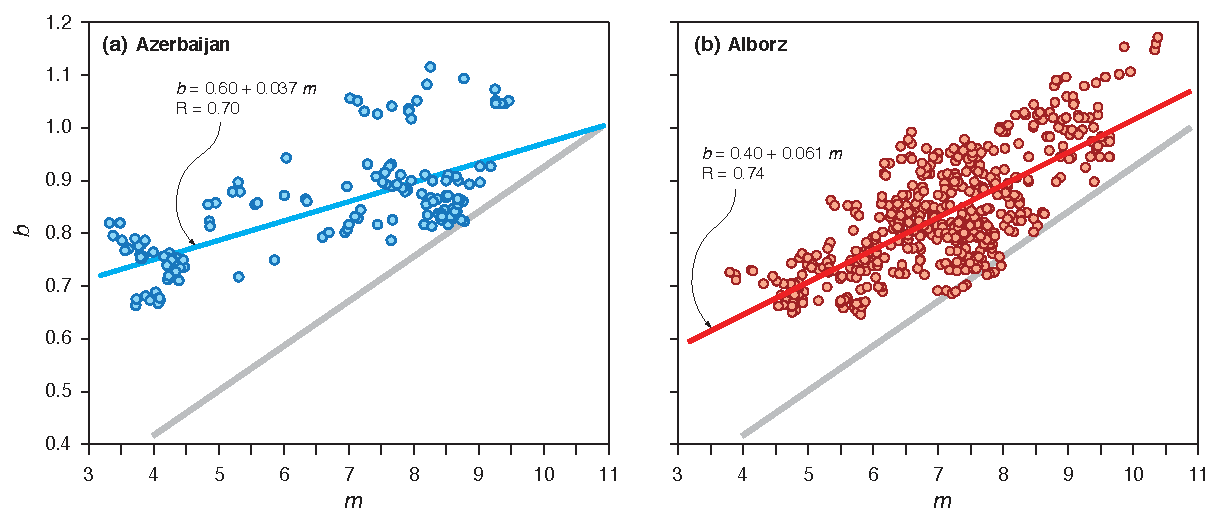
\includegraphics[width=\textwidth]{figures/pdf/figure-10} 
	\caption{\myrevision{Correlation between $m$ and $b$ based on the fixed-size windowing analysis done for the regions of Azerbaijan (a) and Alborz (b), along with the linear regressions of each case. While a direct comparison is not appropriate, the universal regression is shown here for reference.}}
	\label{fig:azal-bm}
\end{figure*}

\myrevision{The better correlation observed between $m$ and $b$ for Alborz than for Azerbaijan is further explored in Fig.~\ref{fig:azal-bm}, which presents the condensed (scattered data-point) results for all the values $k$ and $b$ from Fig.~\ref{fig:tc}. The plots in this figure confirm that the values of $m$ and $b$ correlate better for Alborz. Also included in Fig.~\ref{fig:azal-bm}, for reference, is the universal regression. While a direct comparison with the local regressions is not appropriate, the closer proximity of the Alborz trend line to the universal regression line suggests that the larger number of data points improves the quality of the regression, bringing it closer to the universal correlation line. The results for Kopeh Daght, not included here for brevity, show the poorest correlation, likely due to the least amount of data points, which reinforces the point made about the quality of the regression being dependent on a sufficiently large number of data points.}

% OLD MATERIAL
% -----------------------------------------------------------------

% Another aspect of interest is the stability of the data points themselves. Note that as presented in Fig.~\ref{fig:regression}, the analysis of the sequences shown in Fig.~\ref{fig:mag-time} only contribute one data point per region of interest. Furthermore, each data-point comes from sequences that vary significantly in terms of the number of events and seismic parameters (see Table \ref{tab:seismicity}). 

% \myrevision{According to Scholtz (1968) b-value for microfractures in rocks is reported ranging between 0.11 and 2.58. Using different synthetic and real catalog, in this study we cover a broad range from low b-value (synthetics) to high b-value(subduction zone)}. 

% Fig.~\ref{fig:regression} also includes the results of different linear regressions between the $b$-value and the $k$-$M$ slope. Each regression reflects the addition of new data-points from different studies. Note that the regression improves as new data-points are added, which is indicated by the correlation coefficient $R$, also included in the figure. The correlation fitting various regional seismic data was previously pointed out by \citet{Telesca2014}.

% \cmmnt{Note also that the threshold value of $M_c$ is significantly smaller for Azerbaijan than for Alborz or Kopeh Dagh. This is due in part to the fact that the latter two zones were more seismically active in the time period under consideration} 
% \myrevision{In this study due to using windowing method, we consider a very conservative completeness magnitude}. However, according to \citet{Telesca2012}, the threshold magnitude has a minor effect in the graph parameters.

% Moving on, \citet{Telesca2013} observed that the value of the $k$-$M$ slope was not particularly sensitive to the sample size in the sequence---at least not when considering sufficiently large sequences. On the other hand, as we will see below, if the sequence window is sufficiently small, then the $k$-$M$ slope value shows a relative dependence on time and thus provides insight about the variation of the seismicity as the sequence progresses. 

% Note that the results of the whole catalog for each seismic region is different from Fig.~\ref{fig:regression}. In Fig.~\ref{fig:regression} we choose a time dependent completeness magnitude which is conservative and requires inspection. In order to keep uniformity in the random data test we computed the completeness magnitude through GFT for all subsamples and the whole catalog of each seismic region. Determination of completeness magnitude based on the best score of GFT between synthetic catalog and subsamples could be controversial. It is possible to choose very large $M_c$ just because of slightly higher GFT score than smaller magnitudes. This could result in a sequence of data where is not completely a representative of the domain. However, knowing these source of uncertainties, the randomly generated data conforms the fact that the method is fairly robust for the catalog size and completeness magnitude; where we can easily distinguish the 3 seismic region border. There are some outlier data due to subsamples of aftershocks of big earthquakes. These sequences represent different $k-M$ and $b-value$ relationship. These sequences do not represent the dominant seismicity pattern of the region. In the declustered catalog (is not presented here) we do not see these outliers.}

% \cmmnt{
% The comparisons of the regressions, however, indicate that the analysis of the random sub-catalogs leads to a result more in line with the universal results obtained when considering multiple seismic zones. The linear regression of the random sub-catalogs yields the following equation:
% % 
% \begin{equation}
%    	b = 0.045  +0.390 m \, .
% 	\label{eq:iran.bm}
% \end{equation}

% Note that equations (\ref{eq:universal.bm}) and (\ref{eq:iran.bm}) have similar intercepts with the $b$-value axis, and only slightly different slope constants. In this particular case, the analysis for northern Iran leads to a relationship in which the $b$-value increases more rapidly with $m$ than in the case of the regression obtained for the universal data. The similarity between the two equations, however, is a positive sign of the stability of the method.}

% each of the three seismic zones in northern Iran. The time-magnitude sequence is also included for reference. Note that the behavior of the $k$-$M$ slope and the $b$-value is very similar along time for all three zones. \myrevision{Specially in the case of Alborz where because of higher number of events the correlation is easily seen.} This is consistent with the results presented before. We note that there seems to be a correlation between the behavior of the $b$-value in time with the occurrence of some of these larger events. In particular, some of the events in the figure seem to coincide with a drop in the $b$-value. 

% The decline of the $b$-value before large earthquakes has been studied in other regions before \citep[e.g.,][]{Wyss2000, Wyss2006, Schorlemmer2005, Chan2012}. In the context of the visibility graph analysis, \citet{Telesca2016} observed a decrease in <$T_c$> before the large earthquake of the western India earthquake sequence. We recognize, however, that the lack of larger ($M>6$) events in our region of interest in the last decade prevents us from drawing a stronger conclusion on this regard. 




\section{Conclusions}

We studied the seismicity of the three main seismic regions in northern Iran in the time period between January 2005 and December 2015 using an approach based on the visibility graph method. We tested the applicability of this method for the specific region of interest and in reference to previous results from similar studies. The results confirm previous observations about the correlation that exists between the connectivity parameter $k$, the magnitude of the events in the sequence, the slope of this relationship or $k$-$M$ slope, and the $b$-value from the Gutenberg-Richter law. We obtained mathematical expressions for the region of interest as well as for so-called universal data collected from this study and previous additional analysis for other regions as well as data from experiments and found the relationships to have a good level of similarity. This is indicative of the general nature of the relationship between the $k$-$M$ slope and the $b$ value. We also explored the potential relationships that can be drawn from a time-dependent visibility graph analysis and the variation of the seismicity in the region of interest. We found there may be a potential relationship between the the $b$ value and the occurrence of earthquakes as well as with the graph's mean interval connectivity time parameter <$T_c$>, but additional research in regions with stronger events may be necessary before drawing stronger conclusions in this regard. The method used here, nonetheless, seems to provide an alternative and interesting approach to the analysis of the seismicity of a region.



\input{Acknowledgements}







% ------------------------------------------------------------------------------


% END-AUTHORS FOR TWO COLUMNS FORMAT
% ------------------------------------------------------------------------------

\makeatletter
\if@twocolumn
    \vspace{3ex}
    \noindent\raggedleft\textit{\textbf{Naeem Khoshnevis\\
Center for Earthquake Research and Information\\
The University of Memphis\\
Memphis, TN 38152, U.S.A.\\
nkhshnvs@memphis.edu\\
~\\
Shima Azizzadeh-Roodpish\\
Ricardo Taborda\\
Department of Civil Engineering, and\\
Center for Earthquake Research and Information\\
The University of Memphis\\
Memphis, TN 38152, U.S.A.\\
~\\
Luciano Telesca\\
Institute of Methodologies for Environmental Analysis\\
National Research Council, Tito, Italy\\}}
\fi
\makeatother

\end{document}
